\documentclass[11pt,a4paper]{article}

% ===== Pakete =====
\usepackage[utf8]{inputenc}
\usepackage[T1]{fontenc}
\usepackage[german,provide=*]{babel}
\usepackage[expansion=false]{microtype}
\usepackage[a4paper,margin=2.5cm]{geometry}
\usepackage{setspace}
\onehalfspacing
\usepackage{graphicx}
\usepackage{booktabs}
\usepackage{csquotes}
\usepackage{enumitem}
\usepackage[round,authoryear]{natbib}
\usepackage{tikz}
\usetikzlibrary{positioning}
\usetikzlibrary{positioning,arrows.meta}
\usepackage{pgfplots}
\pgfplotsset{compat=1.18}
\usepackage[hidelinks]{hyperref}

% ===== Zitierbefehle (Autor-Jahr) =====
% \citet{key}  -> Hiniker et al. (2016)
% \citep{key}  -> (Hiniker et al., 2016)

\begin{document}

% =====================================================================
% DECKBLATT
% =====================================================================
\begin{titlepage}
\centering
\thispagestyle{empty}

\vspace*{1.5cm}

% --- DHBW-Logo oben ---

\includegraphics[width=0.42\textwidth]{DHBW-Logo.png}

\vspace{1.5cm}

% --- Titel mit Trennlinien ---
\rule{\linewidth}{0.4pt}\\[0.6cm]
{\LARGE\bfseries Kontextabhängige Wirksamkeit von\\[0.2em]
Interventionen beim Infinite Scrolling\par}
\vspace{0.5cm}
{\large\itshape Eine Einordnung der Studie \enquote{Scrolling in the Deep}\par}
\vspace{0.6cm}
\rule{\linewidth}{0.4pt}

\vspace{0.5cm}


% --- Einordnung ---
{\normalsize Seminararbeit im Rahmen der Vorlesung\\[0.4em]
\emph{Moderne Programmierkonzepte}\\[0.4em]
Duale Hochschule Baden-Württemberg Mannheim\par}

\vspace{1cm}

% --- Matrikel / E-Mail ---
{\footnotesize
\begin{tabular}{r@{\hskip 1.5em}l}
  Ali Bourbouh  & Matr.-Nr.\ 1215114 \quad alibourbouh2005@gmail.com \\[0.3em]
  Najaf Babayev & Matr.-Nr.\ 3701965 \quad najaf.babayev7@gmail.com \\
\end{tabular}\par}

\vfill

% --- Conference-Logo unten (dezent) ---

\includegraphics[width=0.22\textwidth]{DHBW-Conference.png}\\[0.5cm]
{\small Eingereicht für die\\[0.2em]
\emph{DHBW Conference for Development Paradigms 2026}\par}

\vspace{1cm}

{\small \today\par}

\end{titlepage}


\thispagestyle{empty}
\tableofcontents
\clearpage 

% =====================================================================
% ABSTRACT
% =====================================================================


\begin{abstract}
\noindent
Soziale Medien wie TikTok, Instagram oder Reddit laden Inhalte endlos nach, ohne dass ein
natürlicher Endpunkt entsteht. Dieses Prinzip wird als Infinite Scrolling bezeichnet. Es
hält Nutzende in einem passiven, tranceartigen Zustand, in dem das Zeitgefühl verloren geht
und die bewusste Selbstkontrolle nachlässt. In der Forschung wird dieser Zustand als
normative Dissoziation beschrieben. Viele Apps versuchen, mit Erinnerungen oder festen
Zeitlimits gegenzusteuern. Solche Eingriffe wirken jedoch oft nur kurz, weil sie den
aktuellen Zustand und die Situation der Person nicht berücksichtigen. Häufig lösen sie sogar
einen inneren Widerstand aus, sodass Nutzende die Hinweise einfach wegklicken. Diesen
Widerstand bezeichnet man als Reaktanz.

Die vorliegende Arbeit analysiert und bewertet die Feldstudie von
\citet{meinhardt2025scrolling}, die genau an dieser Stelle ansetzt. Die Studie untersuchte
mit der eigens entwickelten Android-Anwendung \emph{InfiniteScape} bei 72 Personen über
sieben Tage hinweg, wie die jeweilige Situation einer Person die Wirkung eines
Pausen-Hinweises beeinflusst. Gemessen wurden zwei Größen: wie schnell jemand nach dem
Hinweis tatsächlich aufhört zu scrollen (Responsivität) und wie stark der innere Widerstand
gegen den Hinweis ausfällt (Reaktanz).

Die Ergebnisse zeigen, dass die Situation eine messbare, aber nur begrenzte Rolle spielt.
Müdigkeit senkte beispielsweise den Widerstand gegen den Hinweis. Insgesamt erklärten die
untersuchten Situationsfaktoren das Verhalten jedoch nur schwach, da die Unterschiede
zwischen einzelnen Personen stärker ins Gewicht fielen. Die vorliegende Arbeit würdigt die
Studie als wichtigen ersten Schritt hin zu situationsbewussten Interventionen, weist aber
zugleich auf ihre statistischen Grenzen hin.
\end{abstract}

\clearpage
% =====================================================================
% TEIL VON ALI (Person 1): EINLEITUNG
% =====================================================================

\section{Einleitung}
\label{sec:einleitung}

Infinite Scrolling hat sich als das dominierende Design-Prinzip moderner
Social-Media-Plattformen etabliert, indem es Inhalte ohne natürliche Unterbrechung endlos
nachlädt. Ob bei Kurzvideos auf TikTok und Instagram Reels oder beim Durchschauen von
Feeds auf Plattformen wie X und Reddit --- das Interface bietet keinen natürlichen
Stoppeffekt mehr. Betreiber nutzen dieses Design bewusst als sogenanntes
\enquote{Dark Pattern}, um die Verweildauer der Nutzenden zu maximieren und sie in einer
passiven Interaktionsschleife zu halten. Das grundlegende Problem dabei ist, dass dieser
endlose Inhaltsstrom Nutzende in einen tranceartigen, dissoziativen Zustand versetzt, in
dem das Zeitgefühl verloren geht und der Zugriff auf die eigene Willensentscheidung
blockiert wird. Reine Selbstkontrolle reicht oft nicht mehr aus, um das Smartphone
wegzulegen, weshalb dieses unkontrollierte Scrollen in der Forschung nachweislich mit
negativen Gefühlen, Bedauern und einer schlechteren Stimmung in Verbindung gebracht wird.

Der entscheidende Unterschied zu aktiven Smartphone-Tätigkeiten wie dem Verfassen von
Nachrichten oder der gezielten Informationssuche liegt in der Passivität des Infinite
Scrolling. Während aktive Nutzungen klare, inhärente Endpunkte besitzen, fehlt beim
endlosen Wischen jede natürliche Barriere, was den automatisierten Übergang in die
normative Dissoziation begünstigt. Bisherige, rein zeitbasierte Interventions-Apps greifen
hierbei zu kurz, da sie die Nutzung meist starr nach festen Zeitregeln blockieren, ohne den
aktuellen Zustand der Person zu berücksichtigen. Sie ignorieren die herabgesetzte
Willenskraft während der Trance und provozieren dadurch meist nur ein genervtes Wegklicken
der Sperre, anstatt eine nachhaltige Verhaltensänderung zu bewirken.

Während der Einfluss von Kontextfaktoren auf das Nutzungsverhalten bei aktiven
Smartphone-Tätigkeiten bereits Gegenstand wissenschaftlicher Untersuchungen war, bleibt
ihre Rolle beim passiven Infinite Scrolling eine zentrale Forschungslücke. Es fehlt an
empirischer Evidenz darüber, wie situative Bedingungen das Durchbrechen dieser tiefen
Interaktionsschleifen mittels digitaler Eingriffe beeinflussen. Die vorliegende Arbeit
widmet sich genau dieser Lücke, indem sie die Studie von \citet{meinhardt2025scrolling}
analysiert. Im Zentrum steht dabei die Forschungsfrage, wie der spezifische Kontext der
nutzenden Person ihre objektive \emph{Responsivität} und ihre subjektive \emph{Reaktanz}
gegenüber Interventionen während des Infinite Scrolling beeinflusst.

Um diese Fragestellung systematisch zu beantworten, ist die Arbeit wie folgt aufgebaut:
Abschnitt~\ref{sec:literatur} widmet sich dem aktuellen Forschungsstand und bettet das
Problem über eine literaturbasierte Kette von der ersten Generation zeitbasierter
Interventionen bis hin zu den psychologischen und kontextuellen Grundlagen ein.
Abschnitt~\ref{sec:methodik} erläutert die methodische Umsetzung der zugrunde liegenden
Studie von \citet{meinhardt2025scrolling} sowie das Versuchsdesign der Anwendung
\emph{InfiniteScape}. Abschnitt~\ref{sec:ergebnisse} präsentiert die empirischen Ergebnisse
der Untersuchung und analysiert die Haupteffekte sowie Interaktionen der verschiedenen
Kontextfaktoren. Die Arbeit schließt in Abschnitt~\ref{sec:diskussion} mit einer kritischen
Diskussion der Befunde, der methodischen Limitationen sowie einem Ausblick auf zukünftige
Forschungsansätze.

% =====================================================================
% TEIL VON ALI (Person 1): LITERATUR REVIEW
% =====================================================================
\section{Literatur Review}
\label{sec:literatur}

Dieser Abschnitt ordnet die untersuchte Studie in das Forschungsfeld ein. Dazu wird ein
Argumentationsbogen über vier Arbeiten gespannt: von frühen, statischen Interventionen
\citep{hiniker2016mytime} über die psychologische Erklärung ihres Scheiterns
\citep{baughan2022dissociation} und die empirische Bedeutung des Kontexts
\citep{rixen2023loop} bis hin zur untersuchten Studie \citep{meinhardt2025scrolling}, die
diese Stränge zusammenführt.

\subsection{Frühe, statische Interventionen und ihre Grenzen}

Frühe Ansätze zur Regulierung der Smartphone-Nutzung setzten vor allem auf starre,
zeitgesteuerte Limits. Ein zentrales Beispiel dafür ist die App \emph{MyTime} von
\citet{hiniker2016mytime}, die auf das Prinzip des \emph{targeted non-use} abzielte ---
also die gezielte Einschränkung von Apps, die Nutzende selbst als reine Zeitverschwendung
empfinden. Obwohl die Nutzung dieser spezifischen Anwendungen in einer zweiwöchigen
Feldstudie kurzfristig um 21\,\% sank, zeigte sich bei den harten Sperren eine grundlegende
Schwäche: Der automatische \enquote{Timeout}-Bildschirm wurde von den Teilnehmenden in
64\,\% der Fälle einfach ignoriert und weggeklickt. Nur in 6\,\% der Fälle führte der
Hinweis zu einem sofortigen Abbruch der Sitzung. Dieses Verhalten macht deutlich, dass rein
zeitbasierte Interventionen an ihre Grenzen stoßen. Sie agieren völlig kontextblind und
rufen ein Verhalten hervor, das sich im Licht späterer Arbeiten als eine Form von Reaktanz
deuten lässt.

\subsection{Die psychologische Erklärung: normative Dissoziation}

Um zu verstehen, warum solche Barrieren so häufig ignoriert werden, muss die psychologische
Beschaffenheit des Infinite Scrolling genauer betrachtet werden. \citet{baughan2022dissociation}
argumentieren, dass das gedankenlose Scrollen Nutzende passiv in einen Zustand der
sogenannten normativen Dissoziation gleiten lässt. Diesen Begriff übernehmen die Autorinnen
und Autoren dabei ausdrücklich von Butler, die die normative Dissoziation als jene
alltägliche Form der Dissoziation von den klinischen, trauma-basierten Störungsbildern
abgrenzt. Dieser alltägliche Zustand ist durch eine
extreme Verengung des Fokus und ein vermindertes Selbstgewahrsein gekennzeichnet, wodurch
Betroffene oft die Kontrolle über ihre Zeit verlieren. Das entscheidende Problem für
digitale Interventionen liegt darin, dass den Nutzenden in dieser kognitiven Absorption ihre
eigene Willensentscheidung (\emph{volition}) und Handlungsmacht (\emph{agency}) temporär
nicht mehr voll zugänglich sind. Reine Willenskraft reicht für ein Beenden der Sitzung daher
oft nicht aus, da der dafür notwendige Steuerungsmechanismus im Moment des Scrollens
blockiert ist. Allerdings zeigte die Studie auch empirisch, dass die getesteten
Design-Eingriffe die normative Dissoziation signifikant reduzierten und die Trance aktiv
unterbrechen konnten.

\subsection{Die empirische Bedeutung des Kontexts}

Wenn Design-Eingriffe grundsätzlich in der Lage sind, diesen Zustand zu durchbrechen, stellt
sich die Frage, welche Faktoren das Ende einer solchen Schleife im Alltag tatsächlich
herbeiführen. Während \citet{baughan2022dissociation} das psychologische Fundament
lieferten, untersuchten \citet{rixen2023loop} in einer siebentägigen Feldstudie das natürliche
Aufhörverhalten von Nutzenden. Sie stellten fest, dass die Gründe für den Abbruch einer
Social-Media-Sitzung meistens nicht innerhalb der Anwendung liegen, sondern stark vom
allgemeinen Kontext der Person abhängen. Die Autoren unterteilten diese Abbruchgründe
empirisch in vier Hauptkategorien: \emph{Real World} (z.\,B.\ anstehende Aufgaben oder
Gespräche), \emph{Device} (gerätebezogene Auslöser wie Benachrichtigungen, veralteter Inhalt
oder Langeweile innerhalb der App), \emph{Internal} (z.\,B.\ körperliche Bedürfnisse und
Zustände wie Müdigkeit oder Hunger sowie soziale Bedürfnisse) und \emph{Undefined} für nicht
näher spezifizierte Gründe, etwa den bloßen Wechsel zu einer anderen Anwendung. Zudem zeigte
sich, dass reines Infinite Scrolling mit einer schlechteren Stimmung
(niedrigere Valenz) einhergeht. Aus dieser Dominanz des Umfelds leiteten
\citet{rixen2023loop} die zentrale Forderung ab, dass digitale Pausen-Helfer den dynamischen
Kontext der Nutzenden zwingend einbeziehen müssen, statt lediglich sture App-Zeiten zu
erfassen. Die Studie blieb jedoch eine praktische Antwort schuldig, da sie das natürliche
Verhalten lediglich beobachtete, aber keine aktive Intervention testete.

\subsection{Zusammenführung: die untersuchte Studie}

Genau an dieser Schnittstelle setzt das Originalpaper von \citet{meinhardt2025scrolling} an
und schließt die von \citet{rixen2023loop} hinterlassene Forschungslücke, indem es die
geforderte kontextbezogene Intervention empirisch überprüft. Im Rahmen einer siebentägigen
Feldstudie untersuchten die Autoren mithilfe der eigens entwickelten Anwendung
\emph{InfiniteScape}, wie sich der Lebenskontext der Nutzenden auf die Wirksamkeit einer
aktiven Intervention --- eines Popups nach 15 Minuten ununterbrochenen Scrollens ---
auswirkt. Um ein vollständiges und nachhaltiges Bild der Verhaltensänderung zu zeichnen,
führt die Studie zwei zentrale Messgrößen ein: Während die \emph{Responsivität} die
objektive Zeitspanne misst, bis eine Person nach dem Erscheinen des Popups tatsächlich mit
dem Scrollen aufhört, erfasst die \emph{Reaktanz} den subjektiven, inneren Widerstand gegen
den digitalen Eingriff. Durch diesen Ansatz untersucht die Arbeit explorativ, wie verwobene
Kontextfaktoren wie die aktuelle Aktivität, soziale Normen oder die Schläfrigkeit der
Nutzenden das Zusammenspiel aus objektiver Wirkung und psychologischer Abwehr beeinflussen.
Damit liefert das Paper eine direkte Antwort darauf, unter welchen Bedingungen digitale
Interventionen die normative Dissoziation des Infinite Scrolling erfolgreich durchbrechen
können, ohne langfristig an der Reaktanz der Nutzenden zu scheitern.

Dass die Frage nach kontextsensitiven Eingriffen über den engeren Fall des Infinite
Scrolling hinaus an Bedeutung gewinnt, zeigt auch die systematische Literaturübersicht von
\citet{xavier2024notifications}. Sie werten 24~Studien zu den negativen Effekten von
Social-Media-Benachrichtigungen auf die Aufmerksamkeit junger Menschen aus und ordnen unter
anderem das Infinite Scrolling explizit als \enquote{aufmerksamkeitsraubendes} Designmuster
ein, das gezielt psychologische Verwundbarkeiten ausnutzt. Zugleich verweisen sie darauf,
dass rein technische, gerätezentrierte Lösungen häufig zu kurz greifen und ein
Zusammenspiel aus Nutzerkontext, Aufmerksamkeit und Anwendungsgestaltung berücksichtigt
werden muss --- eine Forderung, die den kontextbezogenen Ansatz von
\citet{meinhardt2025scrolling} aus einer breiteren Forschungsperspektive stützt.

% =====================================================================
% TEIL VON PERSON 2 (Najaf): METHODIK
% =====================================================================

\section{Methodik der untersuchten Studie}
\label{sec:methodik}

\subsection{Apparatus}

\citet{meinhardt2025scrolling} entwickelten die native Android-Anwendung
\emph{InfiniteScape}, um die Forschungsfrage zu beantworten. Diese beobachtet das
Scrollverhalten der Teilnehmenden auf sechs ausgewählten Social-Media-Plattformen: Facebook,
Instagram, X, Reddit, TikTok und die Shorts-Funktion von YouTube. Technisch basiert die
Anwendung auf dem Accessibility Service von Android, der es ermöglicht, den jeweils aktiven
Bereich innerhalb einer App auszulesen. So ist es \emph{InfiniteScape} möglich zu erfassen,
ob sich Nutzende beispielsweise im Reels-Feed von Instagram aufhalten oder in einen anderen
Bereich gewechselt haben, wie etwa zu Direktnachrichten. Die Anwendung wertet einen
derartigen Wechsel als Unterbrechung des Scrollvorgangs, und nur ein durchgehender
Aufenthalt im selben Feed wird als ununterbrochenes Infinite Scrolling angesehen. Damit
wurde nur das passive Scrollen erfasst und ausgewertet, während andere Interaktionen wie das
Verfassen von Nachrichten oder das Erstellen von Inhalten bewusst ausgeschlossen wurden.

Wurde über einen Zeitraum von 15 Minuten hinweg ununterbrochenes Scrollen festgestellt,
erschien auf dem Bildschirm ein Overlay mit der Aufforderung, eine Pause einzulegen. Die
Gestaltung basierte auf bereits etablierten Bildschirmzeit-Hinweisen von TikTok und
Instagram. Durch eine Bestätigung konnten Nutzende dieses Overlay wegklicken und das
Scrollen fortsetzen, ohne dass die Anwendung gesperrt wurde. Die Entscheidung für die
15-minütige Schwelle basiert auf zwei vorhergehenden Studien: \citet{terzimehic2022iwishihad}
fanden heraus, dass negative Gefühle in Bezug auf die Smartphone-Nutzung normalerweise nach
etwa 10 bis 20 Minuten auftreten, während \citet{rixen2023loop} in einer früheren Feldstudie
demonstrierten, dass Infinite Scrolling in Sitzungen von etwa 10 Minuten Länge zur
dominierenden Aktivität wird \citep{meinhardt2025scrolling}.

\subsection{Studiendesign, Rekrutierung und Teilnehmende}

Alle interessierten Personen durchliefen eine Registrierungsphase über die
Rekrutierungsplattform Prolific, bevor die eigentliche siebentägige Feldstudie begann. Es
wurden ausschließlich Personen aus den USA berücksichtigt, die ein Android-Smartphone mit
Version~10 oder höher besaßen, da die erforderlichen Berechtigungen für die Anwendung auf
diese Versionen abgestimmt waren und zum Zeitpunkt der Studie über 85\,\% der
US-amerikanischen Android-Nutzer mindestens diese Version verwendeten
\citep{meinhardt2025scrolling}. Ein weiterer Faktor für die weitere Teilnahme war, ob die
befragte Person angab, ihr Scrollverhalten in sozialen Medien zumindest gelegentlich zu
bedauern. Zur Hauptstudie wurden nur jene Personen eingeladen, die dieses Bedauern
bestätigten. Die Autoren begründen diese Vorauswahl mit der Selbstbestimmungstheorie von
\citet{ryan2000selfdetermination}, die besagt, dass intrinsische Motivation eine zentrale
Voraussetzung für eine
erfolgreiche Verhaltensänderung ist. Da Bedauern als Hinweis darauf angesehen wird, dass
Individuen ihr eigenes Scrollverhalten bereits als problematisch empfinden, sollte
gewährleistet werden, dass die Teilnehmenden grundsätzlich aufgeschlossen gegenüber der
getesteten Intervention sind.

\vspace{\baselineskip}
\vspace{\baselineskip}

Von den ursprünglich 460 Personen, die die Registrierungsphase abgeschlossen hatten,
erfüllten 316 dieses Bedauernskriterium und wurden somit für die Hauptstudie zugelassen. In
der Endphase luden 160 Personen die App herunter und beteiligten sich an der siebentägigen
Untersuchung. Datenschutzbedenken, technische Schwierigkeiten beim Herunterladen und die
Herausforderung einer siebentägigen Verpflichtung wurden als häufigste Gründe für die
Entscheidung gegen eine Teilnahme genannt. Um sicherzustellen, dass die Beobachtungsdauer
für alle Teilnehmenden gleich war, wurden zum Schluss 88 Personen ausgeschlossen, die die
vollen sieben Tage nicht absolviert hatten. Die endgültige Stichprobe bestand aus 72
Teilnehmenden (33 Männer, 29 Frauen, 10 nicht-binär) mit einem Durchschnittsalter von 35,50
Jahren (SD~$=10{,}01$) \citep{meinhardt2025scrolling}.

\begin{figure}[htbp]
  \centering
  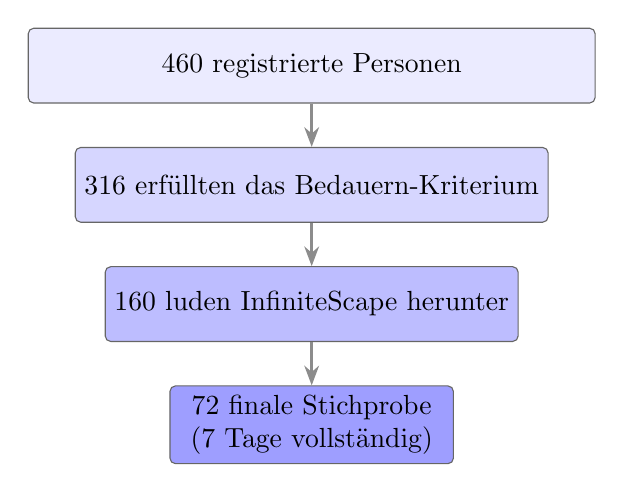
\begin{tikzpicture}[
    node distance=0.55cm,
    box/.style={draw=black!60, rounded corners=2pt, minimum height=0.95cm, align=center, text=black},
    arr/.style={-{Stealth[length=2.5mm]}, draw=black!45, line width=0.9pt}
  ]
    \node[box, minimum width=7.2cm, fill=blue!8]  (a) {460 registrierte Personen};
    \node[box, minimum width=6.0cm, fill=blue!16, below=of a] (b) {316 erfüllten das Bedauern-Kriterium};
    \node[box, minimum width=4.8cm, fill=blue!26, below=of b] (c) {160 luden InfiniteScape herunter};
    \node[box, minimum width=3.6cm, fill=blue!38, below=of c] (d) {72 finale Stichprobe\\(7 Tage vollständig)};
    \draw[arr] (a) -- (b);
    \draw[arr] (b) -- (c);
    \draw[arr] (c) -- (d);
  \end{tikzpicture}
  \caption{Rekrutierungs- und Auswahlprozess der Stichprobe \citep{meinhardt2025scrolling}}
  \label{fig:recruitment-flow}
\end{figure}

\vspace{\baselineskip}

Im Anschluss an die Installation von \emph{InfiniteScape} mussten die Teilnehmenden zunächst
einer von der Ethikkommission der Universität genehmigten Einwilligungserklärung zustimmen
und die notwendigen Berechtigungen für die Anwendung erteilen. Daraufhin gaben sie ihr Alter
und das Geschlecht an, mit dem sie sich am meisten identifizierten. Die App lief während der
gesamten Studie als Android-Hintergrunddienst, was durch ein dauerhaft sichtbares Symbol in
der Statusleiste des Smartphones angezeigt wurde. Die Autoren nehmen an, dass die
Teilnehmenden sich im Laufe der Zeit an dieses Symbol gewöhnten und es ihr natürliches
Scrollverhalten kaum beeinflusste. Die Personen, die an der Registrierungsphase teilnahmen,
wurden mit 0,19~\pounds{} bezahlt. 
In der siebentägigen Hauptstudie erhielten sie zusätzlich für jeden ausgefüllten Fragebogen einen Bonus von 0,5~\pounds{}, was im Durchschnitt 5,20~\pounds{} pro Teilnehmer ausmachte \citep{meinhardt2025scrolling}.

\subsection{Ereignisbasiertes Experience-Sampling}

Zur Erfassung der subjektiven Reaktanz und des aktuellen Kontexts der Teilnehmenden kam die
Experience Sampling Method (ESM) zum Einsatz, ein in der Social-Media-Forschung etabliertes
Verfahren zur wiederholten Befragung von Personen im Alltagskontext. Die Autoren wählten ein
ereignisbasiertes Vorgehen, im Unterschied zu klassischen ESM-Ansätzen, bei denen zu
festgelegten, wiederkehrenden Zeitpunkten Fragebögen ausgelöst werden: Der Fragebogen
tauchte nicht zu einem vorher festgelegten Zeitpunkt auf, sondern genau in dem Augenblick,
in dem eine Person das Infinite Scrolling nach dem Erscheinen der Intervention beendete,
beispielsweise durch das Schließen der App. Die Begründung für diese Entscheidung lautete,
dass ereignisbasierte Ansätze in früheren Studien höhere Antwortraten als periodische
Befragungen lieferten und gleichzeitig garantierten, dass der erfasste Kontext mit dem
relevanten Moment des Scrollabbruchs übereinstimmte \citep{meinhardt2025scrolling}.

Diese Herangehensweise hat jedoch eine methodische Einschränkung zur Folge, die von den
Autoren selbst benannt wird: Der Fragebogen wurde nur bei einem tatsächlichen Abbruch des
Scrollens ausgelöst. Daher wurden Fälle, in denen Teilnehmende die Intervention ignorierten
und weiter scrollten, nicht berücksichtigt. Mit diesem Vorgehen ließ sich der Kontext der
Personen, die die Intervention nicht beachteten, nicht erfassen. Diese durch das
ereignisbasierte Vorgehen bedingte Selektion wird in Abschnitt~\ref{sec:diskussion} als
Limitation wieder aufgegriffen. Trotz dieser Einschränkung
wählten die Autoren das ereignisbasierte ESM, da es sich bereits in ähnlichen Untersuchungen
zur Social-Media-Nutzung als effektiv erwiesen hatte, unter anderem in der Studie von
\citet{rixen2023loop}.

\subsection{Abhängige Variablen: Reaktanz und Responsivität}

\citet{meinhardt2025scrolling} verwendeten kurze Einzel-Item-Messungen anstelle umfangreicher
Fragebogen-Batterien, um die subjektive und objektive Wirkung der Intervention zu erfassen
und der Gefahr einer Ermüdung der Teilnehmenden durch wiederholte Befragungen über sieben
Tage entgegenzuwirken. Trotz der Tatsache, dass Einzel-Item-Messungen grundsätzlich einen
höheren Messfehler besitzen können, sind sie in der Social-Media-Forschung etabliert und
stellen einen angemessenen Kompromiss zwischen Datenqualität und Befragungsaufwand dar. Zur
weiteren Sicherstellung der Datenqualität wurden zufällige Aufmerksamkeitschecks in den
Fragebogen integriert.

Die Reaktanz gegenüber der Intervention wurde als erste abhängige Variable verwendet.
\citet{rains2013reactance} zufolge schränken Interventionen, die auf eine Verhaltensänderung
abzielen, grundsätzlich das
Kontrollgefühl der betroffenen Person ein, was Reaktanz hervorrufen kann. Reaktanz ist nach
\citet{ehrenbrink2020reactance} der innere Widerstand, den eine Person empfindet, wenn sie ihre Wahlfreiheit
bedroht sieht. Im Kontext des Infinite Scrolling kann das Auftreten der Intervention daher
als eine Einschränkung der Entscheidungsfreiheit wahrgenommen werden, da man weiterhin
scrollen darf. Die Reaktanz wurde über die Subskala \emph{Threat} der Reactance Scale for
Human-Computer Interaction (RSHCI) von \citet{ehrenbrink2020reactance} gemessen, die aus fünf Frageitems besteht
und auf einer fünfstufigen Likert-Skala von 1 (\glqq stimme überhaupt nicht zu\grqq{}) bis 5
(\glqq stimme voll zu\grqq{}) erhoben wird. Für jede Beobachtung wurde der Reaktanz-Wert als
Mittelwert über alle fünf Items berechnet \citep{meinhardt2025scrolling}.

Die Responsivität gegenüber der Intervention wurde als zweite, objektive abhängige Variable
erfasst. Sie wurde als die Zeitspanne in Sekunden definiert, die zwischen dem Auftauchen des
Interventions-Overlays und dem tatsächlichen Abbruch des Scrollens verstrich, etwa durch das
Schließen der App oder den Wechsel zu einer anderen, nicht mit Infinite Scrolling
verbundenen Aktion innerhalb derselben App. Außerdem wurde die exakte Uhrzeit jeder
Intervention festgehalten.

Die Nutzung zweier voneinander unabhängiger abhängiger Variablen war für die Untersuchung
essenziell, da eine Maßnahme zwar objektiv wirksam sein kann, indem sie das Scrollverhalten
unterbricht, aber gleichzeitig subjektiv abgelehnt werden könnte. Wie \citet{okeke2018goodvibrations}
demonstrieren, besteht in einem solchen Fall die Gefahr, dass Nutzende trotz kurzfristiger
Verhaltensänderung langfristig zu ihren ursprünglichen Gewohnheiten zurückkehren. Daher war
es erforderlich, neben dem beobachtbaren Verhalten auch die subjektive Wahrnehmung der
Intervention durch die Nutzenden zu dokumentieren \citep{meinhardt2025scrolling}.

\subsection{Die sechs Kontextfaktoren}

\citet{meinhardt2025scrolling} verwendeten sechs verschiedene Kontextfaktoren, um den
aktuellen Kontext der Teilnehmenden zum Zeitpunkt des Scrollabbruchs zu erheben. Diese wurden
jeweils mit etablierten Skalen oder einfachen Ja-Nein-Fragen erfasst. Die gegenwärtige
Aktivität wurde mit der Intervallskala von \citet{samdahl1991leisure} erfasst, die von $-3$ (\glqq definitiv
Freizeit\grqq{}) bis $+3$ (\glqq definitiv nicht Freizeit\grqq{}) reicht und somit angibt, ob
die jeweilige Tätigkeit eher als Freizeit oder als Pflicht angesehen wurde. Die soziale
Situation wurde, angelehnt an die Arbeit von \citet{akpinar2023context}, durch die Frage erfasst, welche
der vorgegebenen Optionen die Personen im Umfeld der Teilnehmenden am besten beschreibe.
Dabei standen drei Antwortmöglichkeiten zur Auswahl: allein, mit Bekannten wie Freunden, Familie oder Kolleginnen und Kollegen sowie mit Fremden.

Eine einfache Ja-Nein-Frage erfasste, ob die Teilnehmenden sich zu Hause befanden.
Multitasking wurde ebenfalls mittels einer Ja-Nein-Frage erfasst, die darauf abzielte,
herauszufinden, ob die Teilnehmenden bei der Nutzung der jeweiligen Anwendung noch eine
andere Tätigkeit ausgeführt hatten. Zur Erfassung der Valenz, sprich der positiven oder
negativen Grundstimmung der Teilnehmenden, kam die Valenz-Dimension der
Self-Assessment-Manikin-Skala (SAM) von \citet{bradley1994sam} zum Einsatz. Diese umfasst fünf
grafische Gesichtsdarstellungen, die verschiedene Stimmungsstufen repräsentieren. Die
Schläfrigkeit der Teilnehmenden wurde schließlich mit der Karolinska Sleepiness Scale (KSS)
erfasst, die von 1 (\glqq extrem wach\grqq{}) bis 9 (\glqq extrem schläfrig\grqq{}) reicht
\citep{meinhardt2025scrolling}.

\subsection{Statistisches Verfahren: Lineare gemischte Modelle}

Zur statistischen Auswertung der Forschungsfrage setzten \citet{meinhardt2025scrolling}
lineare gemischte Modelle (Linear Mixed Models, LMM) ein, jeweils getrennt für die beiden
abhängigen Variablen Reaktanz und Responsivität. Das gewählte Verfahren ist auf die Struktur
der erhobenen Daten zurückzuführen: Weil jede teilnehmende Person im Verlauf der sieben Tage
dauernden Erhebung mehrere Datenpunkte lieferte, sind die einzelnen Beobachtungen nicht
unabhängig voneinander, sondern korrelieren innerhalb derselben Person. Ein typisches
lineares Regressionsmodell würde diese Abhängigkeit ignorieren, was verzerrte und
fälschlicherweise als sicher geltende Schätzungen zur Folge hätte. Um dem entgegenzuwirken,
wurde in allen Modellen ein zufälliger Achsenabschnitt (Random Intercept) pro Teilnehmer
berücksichtigt, der individuelle Unterschiede im Grundniveau jeder Person abbildet und die
Korrelation zwischen wiederholten Messungen derselben Person angemessen modelliert.

Für jede der beiden abhängigen Variablen wurden zwei Modelle erstellt: eines zur Analyse der
Haupteffekte und eines zur Analyse der Interaktionseffekte zwischen den sechs Kontextfaktoren.
Die Haupteffektmodelle wurden mit der Formel Reaktanz bzw.\ Responsivität in Abhängigkeit von
den additiven Effekten der Faktoren Zu~Hause, Aktuelle Aktivität, Schläfrigkeit, Valenz,
Multitasking und Sozialer Situation erstellt. Die Interaktionsmodelle hingegen
berücksichtigten zusätzlich alle möglichen Kombinationen dieser sechs Faktoren, einschließlich
Zwei- und Mehrwege-Interaktionen. Um dem Umstand Rechnung zu tragen, dass mit der Anzahl der
gleichzeitig getesteten Effekte die Wahrscheinlichkeit falsch signifikanter Ergebnisse
zunimmt, wurde das Signifikanzniveau durch eine Bonferroni-Korrektur von dem in der Regel
verwendeten Wert von $\alpha=.05$ auf $\alpha=.025$ herabgesetzt. Die statistische Analyse
wurde mit R (Version~4.3.1) und RStudio (Version~2023.12.1) durchgeführt, während die
grafische Darstellung der Ergebnisse mit Python (Version~3.10.4) erstellt wurde
\citep{meinhardt2025scrolling}.

\section{Ergebnisse}
\label{sec:ergebnisse}

Wie in Abschnitt~\ref{sec:methodik} beschrieben, wurden zur Beantwortung der Forschungsfrage
für jede der beiden abhängigen Variablen zwei lineare gemischte Modelle berechnet: ein
Haupteffektmodell und ein Interaktionsmodell. Bevor die eigentliche Analyse stattfand, wurden
die gesammelten Daten zunächst bereinigt. Elf Datenpunkte wurden entfernt, da die
entsprechenden Teilnehmenden die im Fragebogen enthaltenen Aufmerksamkeitschecks nicht
bestanden hatten. Mit der z-Score-Methode wurden danach Ausreißer bestimmt, wobei ein
Schwellenwert von drei Standardabweichungen vom Mittelwert verwendet wurde. Basierend darauf
wurden acht weitere Datenpunkte der Responsivitätsvariable eliminiert, da die Zeit bis zum
Abbruch des Scrollens hier teilweise über drei Stunden lag, was von den Autoren mit
technischen Schwierigkeiten während dieser Sitzungen erklärt wird. In der weiteren Analyse
wurden nach der Bereinigung 927 Datenpunkte von 72 Teilnehmenden berücksichtigt, was einem
Durchschnitt von 12,88 Datenpunkten pro Person entspricht (SD~$=13{,}02$)
\citep{meinhardt2025scrolling}.

Da die Reaktanz ($W=0{,}95$; $p<.001$) und die Responsivität ($W=0{,}48$; $p<.001$) im
Shapiro-Wilk-Test als nicht normalverteilt identifiziert wurden und die Responsivität zudem
eine ausgeprägte Rechtsschiefe (Schiefe $=3{,}62$) aufwies, wurde eine logarithmische
Transformation der Responsivität durchgeführt, um robustere Schätzungen zu ermöglichen. Dies
führte zu einer Reduktion der Schiefe auf $0{,}782$.

\subsection{Deskriptive Ergebnisse}

\begin{figure}[htbp]
  \centering
  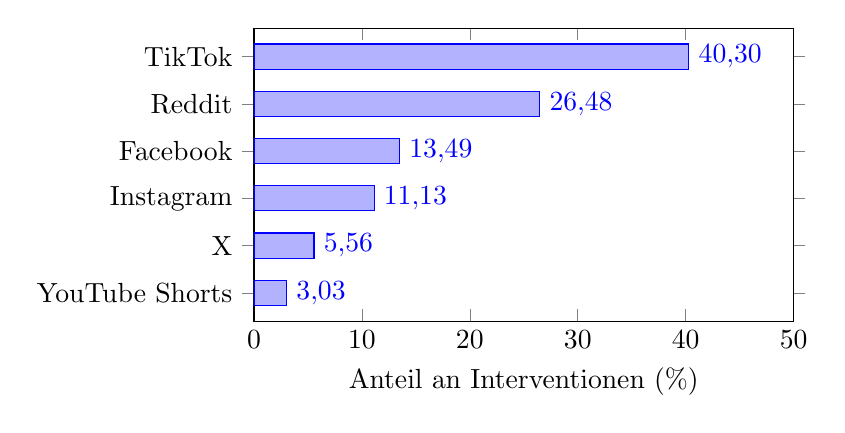
\begin{tikzpicture}
    \begin{axis}[
      xbar, y=0.6cm, bar width=0.32cm,
      xlabel={Anteil an Interventionen (\%)},
      symbolic y coords={YouTube Shorts, X, Instagram, Facebook, Reddit, TikTok},
      ytick=data, xmin=0, xmax=50,
      nodes near coords,
      nodes near coords align={horizontal},
      every node near coord/.append style={
        /pgf/number format/.cd, use comma, fixed, fixed zerofill, precision=2
      },
      enlarge y limits=0.12,
    ]
    \addplot coordinates {(3.03,YouTube Shorts) (5.56,X) (11.13,Instagram) (13.49,Facebook) (26.48,Reddit) (40.30,TikTok)};
    \end{axis}
  \end{tikzpicture}
  \caption{Verteilung der Interventionen nach Plattform \citep{meinhardt2025scrolling}}
  \label{fig:platform-distribution}
\end{figure}

Die durchschnittliche Reaktanz erreichte 3,55 (SD~$=1{,}03$) auf einer Skala von 1 bis 5,
was einem mittleren Niveau entspricht. Die Responsivität wies hingegen große Schwankungen
auf: Teilnehmende beendeten nach dem Auftauchen der Intervention im Schnitt nach 3 Minuten
und 31 Sekunden (SD~$=8$ Minuten und 21 Sekunden) das Scrollen. Die beobachteten Werte
variierten dabei von 0 Sekunden bis zu 67 Minuten und 20 Sekunden. In Bezug auf die
untersuchten Plattformen liegt der größte Anteil der Interventionen auf TikTok (40,30\,\%),
gefolgt von Reddit (26,48\,\%), Facebook (13,49\,\%), Instagram (11,13\,\%), X (5,56\,\%)
und den YouTube Shorts (3,03\,\%) \citep{meinhardt2025scrolling}.

\subsection{Haupteffekte}

Von den sechs untersuchten Kontextfaktoren zeigte sich in den Haupteffektmodellen nur ein
einziger signifikanter Haupteffekt: Bei zunehmender Schläfrigkeit nahm die Reaktanz
gegenüber der Intervention signifikant ab ($t(917)=-3{,}40$; $p<.001$). Die
Pausenaufforderung wurde von müderen Nutzenden als weniger bedrohlich für ihre
Entscheidungsfreiheit wahrgenommen. Die Schläfrigkeit hatte hingegen keinen signifikanten
Einfluss auf die Responsivität. Dies bedeutet, dass müde Personen die Intervention zwar eher
innerlich akzeptierten, jedoch nicht automatisch schneller mit dem Scrollen aufhörten. Bei
den fünf anderen Kontextfaktoren (aktuelle Aktivität, soziale Situation, zu Hause,
Multitasking und Valenz) konnten keine signifikanten Haupteffekte auf Reaktanz oder
Responsivität festgestellt werden.

Hier ist eine methodische Einschränkung zu berücksichtigen, auf die die Autoren ausdrücklich
hinweisen: Aufgrund der Entdeckung signifikanter Interaktionseffekte in den
Interaktionsmodellen (Modell~2 für Reaktanz und Modell~4 für Responsivität) ist eine
eigenständige Interpretation der Haupteffekte, die in diesen beiden Modellen ebenfalls
berechnet wurden, nicht zulässig. Wenn eine Interaktion vorliegt, ist die Beziehung zwischen
einer unabhängigen und einer abhängigen Variablen von einer dritten Variablen abhängig; eine
isolierte Betrachtung des Haupteffekts würde diese Abhängigkeit verschleiern und zu
Fehlinterpretationen führen. Valide interpretierbare Haupteffekte beziehen sich daher
ausschließlich auf die reinen Haupteffektmodelle (Modell~1 und Modell~3)
\citep{meinhardt2025scrolling}.

\subsection{Modellvergleich}
\label{sec:modellvergleich}

Bevor die einzelnen Interaktionseffekte betrachtet werden, ist zu klären, ob die zusätzliche
Komplexität der Interaktionsmodelle im Vergleich zu den einfacheren Haupteffektmodellen
überhaupt gerechtfertigt ist. Hierzu wurden Likelihood-Ratio-Tests
vorgenommen. Bei der Reaktanz ergab sich durch die Einbeziehung von Interaktionseffekten eine
signifikante Verbesserung der Modellanpassung ($\chi^2(60)=83{,}848$; $p=.023$). Bei der
Responsivität fiel diese Verbesserung hingegen knapp nicht signifikant aus
($\chi^2(60)=78{,}265$; $p=.057$), was bedeutet, dass der zusätzliche Erklärungsgewinn der
Interaktionseffekte hier die höhere Modellkomplexität nicht eindeutig rechtfertigt. In der
Summe war der durch die Modelle erklärte Varianzanteil gering: Die marginalen $R^2$-Werte
variierten je nach Modell von $0{,}0072$ bis $0{,}07$, was darauf hinweist, dass die
analysierten Kontextfaktoren nur einen geringen Teil der beobachteten Unterschiede in
Reaktanz und Responsivität erklären konnten \citep{meinhardt2025scrolling}. Dieser Befund ist
für die Einordnung der nachfolgend berichteten Interaktionseffekte zentral und wird dort
wieder aufgegriffen.

\subsection{Interaktionseffekte}

Bei der Reaktanz wurden keine signifikanten Interaktionseffekte der Kontextfaktoren
beobachtet. In Bezug auf die Responsivität wurden hingegen fünf signifikante
Zwei-Wege-Interaktionen und eine signifikante Drei-Wege-Interaktion identifiziert
\citep{meinhardt2025scrolling}.

Bevor die einzelnen Interaktionseffekte im Detail beschrieben werden, ist eine Einschränkung
zu nennen: Der in Abschnitt~\ref{sec:modellvergleich} berichtete Modellvergleich ergab für die
Responsivität keine signifikante Verbesserung des Interaktionsmodells gegenüber dem
Haupteffektmodell ($\chi^2(60) = 78{,}265$; $p = {,}057$). Die im Folgenden beschriebenen
Effekte sind somit statistisch nicht abgesichert und als explorative Tendenzen, nicht als
robuste Befunde zu interpretieren \citep{meinhardt2025scrolling}.

Die erste bedeutende Interaktion fand zwischen Valenz und sozialer Situation in der
Anwesenheit von Fremden statt ($t(857)=-2{,}51$; $p=0{,}012$). Die Stimmung der
Teilnehmenden hatte, wenn sie allein waren, kaum Auswirkungen auf deren Reaktionszeit. In
Anwesenheit von Fremden hingegen nahm die Responsivität mit steigender Valenz deutlich zu:
In dieser Situation reagierten Personen mit besserer Stimmung merklich schneller auf die
Intervention als solche mit schlechterer Stimmung.

Auch zwischen Schläfrigkeit und der sozialen Situation bei Anwesenheit von Fremden zeigte
sich eine ähnliche Wechselwirkung ($t(857)=-2{,}41$; $p=0{,}016$). Während eine zunehmende
Schläfrigkeit die Reaktionszeit nur moderat verlangsamte, führte sie in Anwesenheit von
Fremden zu einer deutlich stärkeren Verkürzung der Reaktionszeit. Es liegen jedoch keine
Beobachtungsdaten vor, die stark erhöhte Schläfrigkeit in Kombination mit der Anwesenheit
von Fremden betreffen. Daher kann dieser Aspekt der Interaktion nicht abschließend
interpretiert werden.

Zudem wurde eine signifikante Wechselwirkung zwischen Valenz und Multitasking festgestellt
($t(857)=-2{,}48$; $p=0{,}013$). Wenn Teilnehmende während des Scrollens noch eine andere
Tätigkeit ausführten, nahm die Responsivität mit einer höheren Valenz zu. Ohne eine solche
Nebentätigkeit trat jedoch das Gegenteil ein: In diesem Fall nahm die Responsivität mit
steigender Valenz ab, was bedeutet, dass Personen in besserer Stimmung langsamer auf die
Intervention reagierten als solche in schlechterer Stimmung.

Auch zwischen der Valenz und dem Faktor Zu~Hause gab es eine bedeutende Interaktion
($t(857)=-3{,}17$; $p=0{,}002$). Waren die Teilnehmenden zu Hause, änderte sich ihre
Responsivität bei steigender Valenz nur geringfügig, während eine niedrige Valenz die
Reaktionszeit tendenziell verlängerte. Wenn die Teilnehmenden nicht zu Hause waren,
resultierte eine höhere Valenz in einer deutlich kürzeren Reaktionszeit.

Außerdem ergab sich eine bedeutende Wechselwirkung zwischen dem Faktor Zu~Hause und
Multitasking ($t(857)=-2{,}67$; $p=0{,}008$). Die Reaktionszeit zu Hause blieb unabhängig
davon, ob die Teilnehmenden gleichzeitig eine andere Aufgabe erledigten, nahezu konstant.
Dagegen bewirkte Multitasking außerhalb des Zuhauses eine merkliche Beschleunigung der
Reaktion auf die Intervention.

Eine signifikante Drei-Wege-Interaktion zwischen den Faktoren Zu~Hause, Valenz und
Multitasking wurde schließlich festgestellt ($t(857)=2{,}77$; $p=0{,}006$). Diese fasst die
beiden zuvor beschriebenen Interaktionen zusammen und deutet darauf hin, dass das
Zu-Hause-Sein einen stabilisierenden Einfluss hat: In der eigenen Wohnung ist die
Responsivität weitgehend unabhängig von Valenz und Multitasking auf einem ähnlichen Niveau,
während außerhalb des Zuhauses sowohl die Stimmung als auch eine parallele Tätigkeit einen
deutlich stärkeren Einfluss auf die Reaktionsgeschwindigkeit der Teilnehmenden haben
\citep{meinhardt2025scrolling}.

\begin{table}[htbp]
  \centering
  \caption{Signifikante Effekte der linearen gemischten Modelle}
  \label{tab:lmm-results}
  \begin{tabular}{@{}llrl@{}}
    \toprule
    Modell & Effekt & $t$ (df) & $p$ \\
    \midrule
    M1: Haupteffekte Reaktanz      & Schläfrigkeit                          & $-3{,}40$ (917) & $< {,}001$ \\
    M2: Interaktion Reaktanz       & \multicolumn{3}{l}{keine signifikanten Interaktionen} \\
    M3: Haupteffekte Responsivität & \multicolumn{3}{l}{keine signifikanten Haupteffekte} \\
    M4: Interaktion Responsivität  & Valenz $\times$ Fremde                 & $-2{,}51$ (857) & $= {,}012$ \\
                                    & Schläfrigkeit $\times$ Fremde          & $-2{,}41$ (857) & $= {,}016$ \\
                                    & Valenz $\times$ Multitasking           & $-2{,}48$ (857) & $= {,}013$ \\
                                    & Valenz $\times$ Zu Hause               & $-3{,}17$ (857) & $= {,}002$ \\
                                    & Zu Hause $\times$ Multitasking         & $-2{,}67$ (857) & $= {,}008$ \\
                                    & Zu Hause $\times$ Valenz $\times$ Multitasking & $2{,}77$ (857) & $= {,}006$ \\
    \bottomrule
  \end{tabular}
  \begin{minipage}{0.9\textwidth}
    \footnotesize\vspace{2mm}
    \emph{Anmerkung:} Bonferroni-korrigiertes Signifikanzniveau $\alpha = {,}025$. Marginale
    $R^2$ variierten zwischen $0{,}0072$ und $0{,}07$ \citep{meinhardt2025scrolling}.
  \end{minipage}
\end{table}

Insgesamt deuten diese Resultate darauf hin, dass die einzelnen Kontextfaktoren nicht
unabhängig voneinander die Reaktionsgeschwindigkeit der Nutzenden auf die Intervention
beeinflussen, sondern dass ihr Zusammenspiel entscheidend ist. Angesichts des nicht
signifikanten Modellvergleichs für die Responsivität ist dieses Zusammenspiel jedoch als
explorativer Hinweis und nicht als abgesicherter Nachweis zu verstehen.

% =====================================================================
% TEIL VON ALI (Person 1): DISKUSSION
% =====================================================================

\section{Diskussion und Zusammenfassung}
\label{sec:diskussion}

\subsection{Stärken}

Ein wesentlicher methodischer Vorteil der Untersuchung von \citet{meinhardt2025scrolling}
liegt in ihrer hohen ökologischen Validität. Durch die Durchführung als siebentägige
Feldstudie im realen Alltag der Teilnehmenden wurde das tatsächliche Scroll- und
Abbruchverhalten auf den eigenen Smartphones erfasst. Dies minimiert den klassischen
Hawthorne-Effekt, da sich situative Kontexte --- wie das Scrollen im Bett oder während der
Arbeitszeit --- in einer künstlichen Laborumgebung ohnehin nicht realitätsgetreu simulieren
lassen. Zudem erweist sich die synchrone Erfassung von objektiver \emph{Responsivität} und
subjektiver \emph{Reaktanz} als wissenschaftlich gewinnbringend. Erst diese methodische
Kombination verhindert eine Fehlinterpretation der Daten: Eine rein zeitbasierte Messung
würde den echten Stopp der Sitzung zwar als Erfolg werten, den potenziell parallel
entstehenden inneren Widerstand der Nutzenden jedoch vollständig übersehen.

\subsection{Schwächen}

Trotz dieser methodischen Stärken weist die Untersuchung von \citet{meinhardt2025scrolling}
auch kritische Schwachstellen auf, welche die Aussagekraft der Befunde einschränken. Ein
zentrales statistisches Problem liegt in der geringen erklärten Varianz (marginale
$R^2$-Werte) der Kontextfaktoren. Da diese Faktoren nur einen minimalen Teil des Verhaltens
erklären, bleibt die Kernbehauptung der Studie --- dass der Kontext die Reaktion auf Popups
maßgeblich steuert --- theoretisch angreifbar, da interindividuelle Unterschiede zwischen
den Personen offenbar schwerer wiegen. Verschärft wird diese Einschränkung dadurch, dass das
Interaktionsmodell für die Responsivität im Modellvergleich keine signifikante Verbesserung
gegenüber dem reinen Haupteffektmodell erbrachte ($p=.057$; siehe
Abschnitt~\ref{sec:modellvergleich}). Die in Abschnitt~\ref{sec:ergebnisse} berichteten
Interaktionseffekte auf die Responsivität sind daher statistisch nicht abgesichert, was die
zentrale Aussage der Studie zusätzlich relativiert.
Bemerkenswert ist, dass die Autoren die geringe erklärte Varianz
selbst benennen und einräumen, dass individuelle Unterschiede einen
ausgeprägteren Einfluss haben könnten als die untersuchten Kontextfaktoren.

Eine weitere
Einschränkung betrifft die Selektion der Stichprobe nach dem Kriterium des
\enquote{Bedauerns}: Bewusst wurden ausschließlich Personen einbezogen, die ihre eigene
Nutzung bereuen, da diese laut Selbstbestimmungstheorie überhaupt erst die intrinsische
Motivation mitbringen, auf Interventionen zu reagieren. Diese begründete Entscheidung
schränkt jedoch die Repräsentativität ein, da Nutzende, die ohne Reuegefühl scrollen,
fehlen. Denkbar wäre zudem, dass diese reue-geneigten Nutzenden die Intervention zugleich
als moralischen Zeigefinger empfinden, was die gemessene Reaktanz beeinflussen könnte.

Eine zusätzliche Limitation ergibt sich aus dem ereignisbasierten Sampling-Design (vgl.\
Abschnitt~\ref{sec:methodik}): Da der Fragebogen nur bei einem tatsächlichen Scrollabbruch
ausgelöst wurde, blieb der Kontext jener Teilnehmenden, die die Intervention ignorierten und
weiterscrollten, vollständig unerfasst. Diese selektive Erfassung stellt einen potenziellen
Selektionsbias dar, da nur Fälle beobachtet wurden, in denen die Intervention überhaupt
wirkte.

Ein weiterer Punkt betrifft das Fehlen einer Kontrollgruppe ohne Intervention. Da alle
Teilnehmenden dem Pausen-Popup ausgesetzt waren, lässt sich nicht kausal nachweisen, dass
das beobachtete Abbruchverhalten tatsächlich auf die Intervention und nicht auf ohnehin
eintretende, kontextbedingte Abbruchgründe zurückgeht --- ein Punkt, den die Autoren als
möglichen Baustein künftiger Studien selbst ansprechen.

Hinzu kommt schließlich, dass die technisch bedingte Beschränkung auf US-amerikanische
Android-Nutzende die Übertragbarkeit der Ergebnisse zusätzlich einschränkt.

\subsection{Gesamtbewertung und Ausblick}

Unterm Strich leistet die Untersuchung von \citet{meinhardt2025scrolling} einen wichtigen
empirischen Pionierbeitrag, da sie die in der Literatur wiederholt geforderte
Kontext-Perspektive erstmals im Rahmen eines echten Interventions-Experiments überprüft.
Dieser Pionierstatus ist jedoch klar von der Belastbarkeit der Einzelbefunde zu trennen:
Angesichts der durchweg geringen erklärten Varianz und des nicht signifikanten
Modellvergleichs für die Responsivität liefert die Studie weniger einen gesicherten Nachweis
kontextabhängiger Wirkungen als vielmehr ein methodisch wertvolles Fundament, auf dem
weitere Arbeiten aufsetzen können.
Trotz dieser Einschränkungen liefert das Paper durch die Kombination von Reaktanz- und
Responsivitätsmessung ein neues Instrumentarium für die Gestaltung digitaler
Pausen-Helfer. Aufgrund der kurzen Studiendauer von sieben Tagen und der geringen
marginalen Effekte sind die Befunde jedoch eher als fundierter Ausgangspunkt denn als
abschließender Beweis zu verstehen. Künftige Forschungsarbeiten müssen darauf aufbauen und
über längerfristige Untersuchungszeiträume, eine Kontrollgruppe ohne Intervention sowie
vielfältigere Stichproben prüfen, ob
kontextsensitive Interventionen auch dauerhaft der psychologischen Desensibilisierung der
Nutzenden standhalten können.

Für die Praxis lässt sich aus den Befunden vorsichtig ableiten, dass digitale Pausen-Helfer
nicht nach einem starren Zeitschema, sondern situationsabhängig eingreifen sollten. So legt
der gefundene Zusammenhang zwischen Schläfrigkeit und gesunkener Reaktanz nahe, dass abendlich
müde Nutzende Interventionen eher akzeptieren, ohne allerdings zwingend schneller aufzuhören; ein
gestuftes, sich langsam verstärkendes Eingreifen könnte hier wirksamer sein als eine einmalige
harte Sperre. Ebenso deutet die stabilisierende Rolle des Faktors Zu~Hause darauf hin, dass
Interventionen im häuslichen Umfeld gezielter gestaltet werden müssen. Solche Empfehlungen sind
aufgrund der genannten statistischen Einschränkungen jedoch als Hypothesen für künftige
Studien und nicht als gesicherte Gestaltungsregeln zu verstehen.

\subsection{Zusammenfassung}

Die vorliegende Arbeit rekonstruierte das Problem des Infinite Scrolling, das als
manipulatives Design-Prinzip Nutzende passiv in eine normative Dissoziation führt, an der
herkömmliche, rein zeitbasierte Interventionen meist wirkungslos scheitern. Um diese Lücke
zu schließen, wurde die Feldstudie von \citet{meinhardt2025scrolling} analysiert, die über
die Anwendung \emph{InfiniteScape} bei 72 Teilnehmenden über sieben Tage hinweg
untersuchte, wie der dynamische Lebenskontext die objektive Responsivität und subjektive
Reaktanz gegenüber einem Pausen-Popup beeinflusst. Die empirischen Befunde verdeutlichen,
dass der Kontext eine messbare, jedoch stark verwobene Rolle spielt: Während eine höhere
Schläfrigkeit die Reaktanz senkt, hängen die Effekte auf die Responsivität maßgeblich von
komplexen Interaktionen der Faktoren ab und fallen insgesamt schwächer aus als die
interindividuellen Unterschiede der Nutzenden.

Ordnet man diese Befunde in die in Abschnitt~\ref{sec:literatur} skizzierte Forschungslinie
ein, so bestätigt die Studie die von \citet{rixen2023loop} formulierte Forderung nach
kontextsensitiven Eingriffen zwar dem Grundsatz nach, zeigt aber zugleich, wie schwer sich
der Kontexteinfluss empirisch dingfest machen lässt: Die geringe erklärte Varianz und der
nicht signifikante Modellvergleich für die Responsivität machen deutlich, dass der Schritt
von der beobachteten Relevanz des Kontexts (Rixen et al.) hin zu seiner gesicherten
Wirksamkeit in einer aktiven Intervention noch nicht vollständig gelungen ist. Aus eigener
Sicht liegt der Hauptwert der Arbeit daher weniger in den konkreten Einzeleffekten als in
der methodischen Innovation, objektive Responsivität und subjektive Reaktanz erstmals
gemeinsam und im Feld zu erheben.

Offen bleiben mehrere Fragen, an denen künftige Forschung ansetzen sollte: ob sich die
Kontexteffekte über längere Zeiträume und in kulturell vielfältigeren, plattform- wie
betriebssystemübergreifenden Stichproben stabilisieren lassen, ob eine Kontrollgruppe ohne
Intervention die kausale Rolle des Popups belegen kann und ob eine objektive
Kontexterfassung die auf Selbstbericht beruhenden Befunde bestätigt. Als theoretischer und
praktischer Pionierbeitrag liefert die Untersuchung damit einen fundierten Ausgangspunkt für
zukünftige, kontextsensitive Design-Ansätze, markiert aufgrund der geringen erklärten
Varianz und des kurzen Untersuchungszeitraums jedoch keinen abschließenden Beweis.

\clearpage

% ===== Literatur =====
\bibliographystyle{plainnat}
\addcontentsline{toc}{section}{Literatur}
\bibliography{literatur}

\end{document}